% ---------------------------------------------------
%
% Trabajo de Fin de Grado. 
% Author: Laura Padrón Jorge. 
% Capítulo: La aplicacion BulletPoint. 
% Fichero: Cap4_TheApplication.tex
%
% ----------------------------------------------------
%

\chapter{La aplicación BulletPoint} \label{chap:LaAplicacion} 

Basándonos en los casos de uso revisados en el capítulo anterior, en este capítulo se discutirán los casos de uso que han sido elegidos e implementados en la aplicación \BulletPoint{}. Comentaremos la aplicación centrándonos en el desarrollo de la misma, así como  en diferentes partes a destacar del código que puedan resultar interesantes.


\section{Casos de uso elegidos}

Como ya hemos mencionado previamente, estos casos de uso se incluyen como parte de la aplicación que se ha desarrollado en este TFG, donde cada caso de uso se considera un módulo. La integración de cada uno de estos módulos con el resto de la aplicación se ha realizado mediante el desarrollo de un menú de funcionalidades donde es posible seleccionar qué acción se desea. Para almacenar la información necesaria para algunos módulos, se ha introducido un menú adicional de ajustes. Estos datos se utilizan entre otras cosas para identificar al usuario y confirmar ciertas acciones o dejar constancia de otras. 


A continuación se desglosarán los distintos casos de uso en los que tendremos que pensar de ahora en adelante como módulos, junto con la explicación del caso de uso y su funcionamiento se incluirán algunos de los detalles más importantes de la implementación de cada uno.

\subsection{Localización de transporte público, horarios e \\información de la parada}

\subsubsection{Objetivo}


El objetivo de este caso de uso es el conocer, en tiempo real, qué autobuses pasan por la parada en la que nos encontramos, hacia dónde se dirigen, y cuánto tiempo falta para que lleguen a la parada. En caso de necesidad de información adicional, la aplicación está preparada para remitirnos a navegar por la página web \cite{URL::titsa} de la empresa Transportes interurbanos de Tenerife, S.A.(TITSA), donde podemos ver datos adicionales sobre el autobús seleccionado.

\begin{figure}[H]
	\centering
	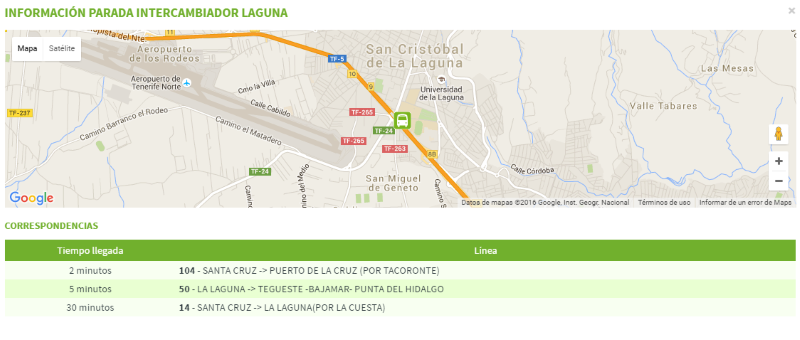
\includegraphics[width=0.7\linewidth]{titsaMap}
	\caption{Información mostrada por TITSA actualmente en su página web.}
	\label{fig:MapaTitsa}
\end{figure}

\subsubsection{Despliegue}

En este caso, sería necesario colocar un beacon en cada parada de autobuses. De esta manera cada parada de autobús queda identificada por un beacon. Si el usuario se encuentra cercano a dos paradas, la aplicación considera que le interesa la información de la parada más cercana a su posición y le proporcionará información únicamente de esta parada con el objetivo de no confundir al usuario.

\subsubsection{Funcionamiento}


Mediante el uso de los beacons, permitimos a la aplicación identificar en que parada se encuentra el usuario. La aplicación asocia la MAC \ref{el:mac} de un beacon con el número identificativo de la parada. Este número identificativo de la parada es lo que utiliza TITSA para identificar sus paradas en la API y en toda su web. 


La aplicación ha sido programada enlazando los números identificativos de la parada con la dirección MAC de los beacons. En el listado \ref{code:beaconbusstop} se puede apreciar como se relaciona cada MAC con el número identificativo de la parada.


\lstinputlisting[float, floatplacement=H,caption={\textit{BusBeaconStop}. Esta clase contiene la información que asocia cada MAC con el ID de la parada de TITSA. Añadir un nuevo beacon a una parada implica añadir un nuevo elemento a \textit{stopsMapId}.}, label={code:beaconbusstop}]
{listings/BeaconBusStop.java} %% LISTING


Cuando la aplicación detecta un beacon, es capaz de reconocer la parada en la que se encuentra el usuario. Una vez la aplicación conoce los datos de la parada, se procede a realizar dos peticiones de comunicación con el servicio de TITSA: 


\begin{itemize}
\item La primera petición se hace sobre la API de TITSA y nos proporciona la información de los autobuses y el tiempo restante para que llegue dicho autobús a la parada. Cabe destacar que para poder utilizar esta API se contactó con TITSA, cuyo personal nos proporcionó una API KEY para poder trabajar con ella. Podemos ver el método principal en el listado \ref{code:basedOnLineNumber}.
\item La segunda petición se realiza sobre la web de TITSA directamente. El objetivo de esta petición es obtener para cada autobús la información de su recorrido. Para ello se obtiene el código de la página en HTML extrayendo la información relativa a su itinerario. La información no se encuentra en un formato óptimo en algunos casos, pero esta información proviene de TITSA y ofrece una información necesaria para usuario. 
\end{itemize}


Aparte de esta información, por cada autobús se incluye un enlace a modo de botón que remite al usuario a la página web de TITSA con el identificador de la línea. Así el usuario puede obtener más información adicional en caso de precisarla.

\lstinputlisting[float, floatplacement=H, caption={La clase \textit{Arrival} donde quedan contenidos los datos de cada llegada.}, label={code:arrival}]
{listings/Arrival.java} %% LISTING

En un principio nuestra idea era utilizar simplemente la API de TITSA, puesto que se creía que proporcionaría toda esta información; sin embargo, en algunos casos los destinos no se correspondían con la realidad y las rutas aparecían erróneas. Ante esta situación, se contactó con personal de  TITSA involucrado en el desarrollo de esta API quien nos comentó que esto ocurría en algunos casos por la manera en la que estaba planteada la API.


La solución que se adoptó, fue utilizar ambos métodos para obtener la información completa. Dichos métodos serán desglosados a continuación: 


En el primer método, utilizando una librería de peticiones HTTP, se envía una consulta por GET a la API de TITSA que devuelve una respuesta en XML. Esta respuesta se parsea con un handler de XML (véase Listado \ref{code:handler}). 
\vspace{5mm}
\lstinputlisting[float, floatplacement=H,caption={El handler se encarga de transformar el fichero XML en elementos de tipo \textit{Arrival} (véase Listado \ref{code:arrival}).}, label={code:handler}]
{listings/XmlHandler.java} %% LISTING


Al mismo tiempo, se inicia la petición a la página de TITSA y utilizando la librería Jsoup \cite{URL::Jsoup}, se obtiene el contenido de la página web. De este contenido en HTML, recopilamos únicamente el recorrido de los autobuses y el resto se descarta como podemos ver en el listado \ref{code:jsoup}. Esta petición es bastante más pesada que la del XML previa, ya que tiene que obtener todo el contenido de la página web en la que aparece el desglose del itinerario en formato HTML. El parseo de la página también es más lento que en el paso previo, ya que debe ir elemento por elemento iterando en los elementos hijos del HTML.

\lstinputlisting[float, floatplacement=H,caption={El método \textit{getTimetablesBasedOnLineNumber()} del cliente de TITSA se encarga de obtener los datos de su API y devolver una lista de llegadas.}, label={code:basedOnLineNumber}]
{listings/HttpClientTitsa.java} %% LISTING

\lstinputlisting[float, floatplacement=H,caption={El método \textit{getCorrectRoute()} nos permite obtener el itinerario correcto del autobús.}, label={code:jsoup}]
{listings/HttpClientTitsaJsoup.java} %% LISTING

Utilizando ambos conjuntos de datos, se va creando una estructura con los mismos, donde se almacena la información sobre cada elemento. En última instancia vamos añadiéndolos a la vista utilizando un adaptador y una estructura para visualizarlos.

\begin{figure}[H]
	\centering
	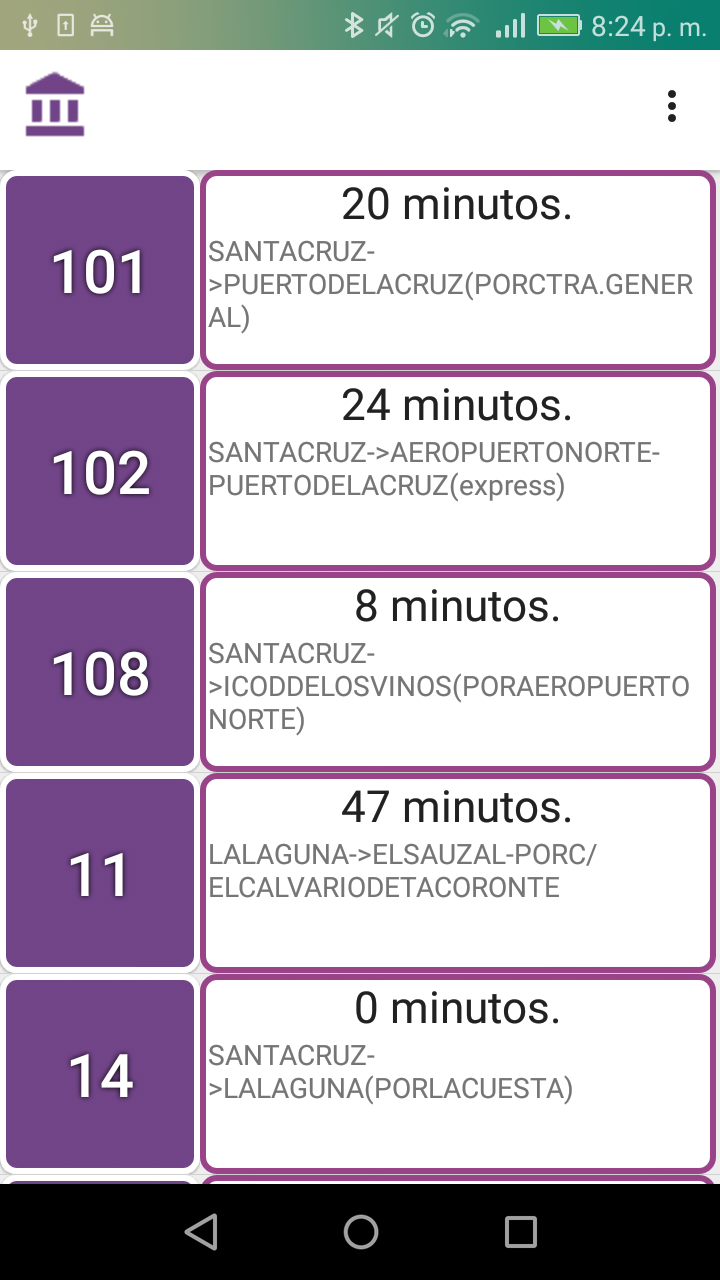
\includegraphics[width=60mm,height=100mm]{Autobuses}
	\caption{\BulletPoint{} permite conocer en tiempo real, autobuses que se acercan a la parada, junto con su destino y tiempo de llegada de la parada identificada por un beacon.}
	\label{fig:autobuses}
\end{figure}

\subsubsection{Dificultades}


Al plantear este caso de uso se han detectado las siguientes dificultades: 

\begin{itemize}
\item A la hora de presentar los datos, la generación de la estructura fue un proceso con el que no se estaba familiarizado y que llevó más tiempo del previsto inicialmente; sin embargo, ha servido de piedra angular para el desarrollo de los demás casos de uso ya que presenta elementos comunes: peticiones, parseo de datos, visualización de listas, etc.
\item Otra dificultad ha sido el no poder obtener todos los datos necesarios con una sola petición y tener que hacer uso de dos peticiones distintas con el tratamiento posterior de los respectivos datos, ya que no eran en absoluto similares.
\end{itemize}


\subsubsection{Ampliación}

Ampliar este caso de uso sólo conllevaría asociar los nuevos identificadores de los beacons a nuevos identificadores de parada. Por ello podemos afirmar que sería relativamente sencillo desplegar una red de beacons en las paradas de autobús de TITSA. 


\subsection{Gestión de eventos e información}

\subsubsection{Objetivo}

El objetivo de este caso de uso sigue siendo el de proporcionar información de eventos e información de interés para el usuario; sin embargo, se ha desligado el módulo de entrada automática, al que hacíamos mención en el análisis previo, ya que en la mayoría de los casos esta funcionalidad no es necesaria.  


\subsubsection{Despliegue}


En este caso, sería necesario colocar un beacon en sitios de interés donde puedan tener lugar eventos. Al mismo tiempo, también es necesaria una fuente de datos donde alojar la información de los eventos. De esta manera cada beacon hace referencia a una fuente de información de eventos. Si el usuario se encuentra cercano a dos beacons, la aplicación considera que le interesa la información del beacon más cercano a su posición. Si se desplaza a otra posición y se acerca a otro beacon, la información sería diferente.

\subsubsection{Funcionamiento}


Mediante el uso de los beacons, permitimos a la aplicación identificar en qué localización se encuentra el usuario. En este caso, hemos utilizado la información RSS del portal web eventosULL \cite{URL::eventsull}. Esta página posee diferentes enlaces RSS que actualmente no están separados por ubicación sino por categorías variadas (ocio, eventos, deportes, tecnologías,etc.). Sin embargo lo hemos tomado como ejemplo porque constituye un portal que ya está en funcionamiento y proporciona información sobre eventos actuales relacionados con la Universidad de la Laguna. 


La aplicación ha sido programada enlazando la dirección MAC de los beacons con diferentes enlaces RSS de la página web de eventos como podemos apreciar en el listado \ref{code:rss}. Al detectar un beacon, se reconoce a qué información queremos acceder y se procede a realizar una petición utilizando el enlace identificado por el beacon: 

\lstinputlisting[float, floatplacement=H, caption={La información de la MAC del beacon queda asociada a un enlace RSS.}, label={code:rss}]
{listings/RssBeaconInfo.java} %% LISTING

La petición se lanza sobre el enlace, el cual nos devuelve un archivo XML que procedemos a tratar para extraer la información que nos interesa. Para no sobrecargar la aplicación con demasiada información del evento, hemos decidido utilizar sólo los datos más relevantes: el título y la fecha del evento. Al mismo tiempo, sobre cada evento se incluye un enlace que, al ser seleccionado, remite a la página web del evento para suministrar información adicional sobre él (localización en un mapa, manera de inscribirse al evento, etc.). Sin embargo, esta información no está disponible para todos los eventos.


En un principio, se planteó el filtrar los eventos para obtener los cercanos a una posición geográfica; sin embargo, no todos los eventos poseen esta información, y sería necesario realizar una petición por cada RSS para obtener los datos y el proceso sería más lento. Si en el futuro se planteara, cada RSS debería relacionarse con la localización del evento.

\begin{figure}[H]
	\centering
	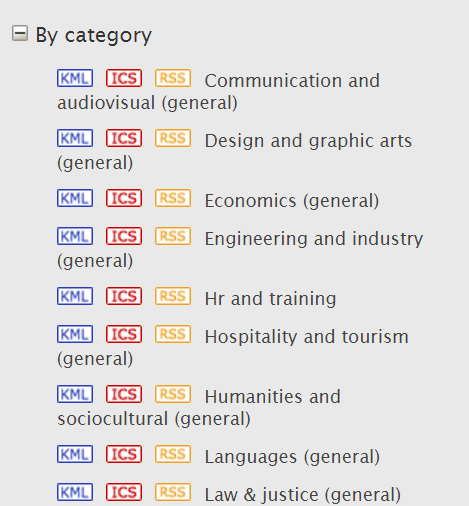
\includegraphics[width=85mm,height=70mm]{eventsRss}
	\caption{Las diferentes categorías de los RSS del portal web de eventos.ull.es}
	\label{fig:eventsRss}
\end{figure}


La petición se realiza utilizando la misma librería de peticiones HTTP que en el caso anterior: se envía una consulta por GET al enlace RSS de la página web de eventosULL el cual nos devuelve una respuesta en XML. Esta respuesta se parsea con un handler de XML para seleccionar únicamente los datos que nos interesan. Esta petición es bastante rápida y genera una vista con la información de los distintos eventos. Cada elemento evento de esta lista es capaz de remitir a la página web de eventosULL para recibir información adicional en caso de estar interesados en el evento en cuestión.

\begin{figure}[H]
	\centering
	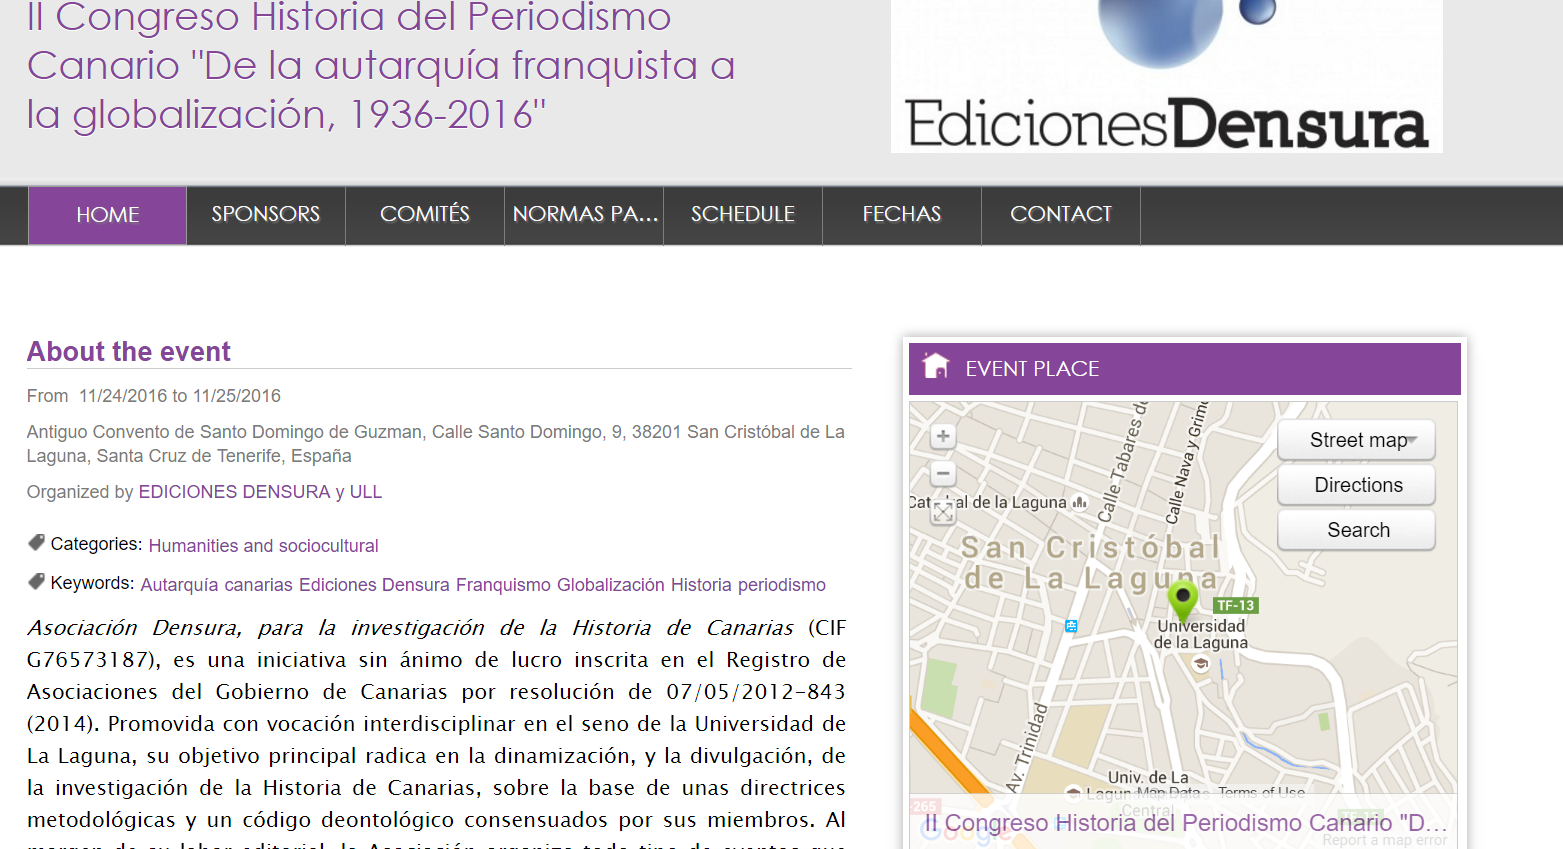
\includegraphics[width=0.7\linewidth]{eventsPage}
	\caption{El portal web de eventos, donde podemos obtener información adicional de un evento concreto.}
	\label{fig:eventsPage}
\end{figure}

\begin{figure}[H]
	\centering
	
\includegraphics[width=60mm,height=100mm]{Eventos}
	\caption{Usando \BulletPoint{} podemos conocer eventos asociados a un RSS del portal web.}
	\label{fig:eventos}
\end{figure}

\subsubsection{Dificultades}


A la hora de implementar este caso de uso no ha habido grandes dificultades. Sin embargo, la fuente de datos no ha sido la óptima, ya que lo ideal hubiese sido poder filtrar los eventos por localización en lugar de por categorías. Aún así, se ha conseguido el objetivo principal de mostrar diferentes eventos en función del beacon detectado.

\subsubsection{Ampliación}


Ampliar este caso de uso sólo conllevaría asociar los nuevos identificadores de los beacons a nuevos identificadores de ficheros RSS. Es por ello que podemos afirmar que sería relativamente sencillo desplegar una red de beacons en diferentes puntos del campus universitario asociados a un RSS. En caso de utilizar otro medio al RSS, sólo habría que adaptar la obtención y la visualización del nuevo contenido, modificando la dirección y añadiendo un nuevo parseo.


\subsection{Control de asistencia}

\subsubsection{Objetivo}

Este caso de uso tiene como objetivo controlar la asistencia de los alumnos a las clases u otro evento que requiera control de asistencia. En un principio se había descartado por las complicaciones que presentaba: 

\begin{itemize}
\item Era necesario tener un servidor en el que poder almacenar la información de las asistencias con la información de los participantes.
\item Se necesitaba un modo de almacenar los datos del usuario para poder identificarle a la hora de registrar la asistencia.
\item El área de acción para registrar la asistencia podía ser variable, sin ser muy exacta. El rango podía salirse del aula o localización de la actividad.
\item Debía de haber algún tipo de control para no registrar asistencias erróneas o fraudulentas.
\end{itemize}

Para solucionar estos problemas se ha optado por las siguientes soluciones: 

Como servidor se ha utilizado \textit{``Couchbase Server"}, una base de datos distribuida no-SQL, orientada a documentos y de código abierto. Por otro lado, se ha configurado en la aplicación móvil una base de datos \textit{``Couchbase Lite"} que sirve de paso intermedio e interactúa con \textit{``Sync Gateway"} para sincronizar los datos de la base de datos del dispositivo al servidor y viceversa.


Para almacenar los datos del usuario, se ha hecho uso de la API de preferencias de Android como podemos apreciar en los listados \ref{code:loadpreferences} y \ref{code:xmlpreferences}, el cual almacena los datos en el dispositivo móvil en un espacio compartido para toda la aplicación. De esta manera, se han almacenado datos como \textit{``Nombre de Usuario"}, \textit{``Número Das"} o \textit{``DNI"}, los cuáles solo serán visibles para el usuario de la aplicación y servirán para registrar las asistencias con estos datos.

\lstinputlisting[float, floatplacement=H, caption={Para cargar la pantalla de preferencias de un fichero XML en el fragmento \textit{Settings}.},label={code:loadpreferences}]
{listings/SettingsActivity.java} %% LISTING

\lstinputlisting[float, floatplacement=H,language=xml, caption={El fichero XML de donde se cargan todas las preferencias.},label={code:xmlpreferences}]
{listings/preferences.xml} %% LISTING

En cuanto al área de acción a partir de la cual es posible registrar la asistencia, se ha optado por establecer un perímetro dentro del aula delimitado por las paredes de la misma, descartando cierto margen y de manera que el aula quede cubierta y los exteriores no se tengan en cuenta. 

\subsubsection{Despliegue}

En este caso, para poder realizar este proceso es necesario utilizar la trilateración \cite{URL::trilateracion} por lo que, es necesario desplegar al menos 3 beacons. Para las pruebas se ha utilizado el aula 2.1 del Edificio de Ingeniería Informática. 

\vspace{5mm}

Estos beacons no tienen que ser necesariamente por aula ya cada beacon cubre un área de 70 metros de radio aproximadamente; teniendo en cuenta que las paredes crean interferencias en la señal, probablemente se podrían utilizar 3 beacons para cubrir dos aulas, pero habría que hacer un estudio de la localización y las interferencias para poder asegurarlo. 

\subsubsection{Funcionamiento}

En cuanto se accede al módulo de asistencia, la aplicación comienza a escanear las inmediaciones buscando beacons. Cuando detecta más de 2 beacons, la aplicación carga la imagen de dicha localización y comprueba que el alumno se encuentra dentro de la zona delimitada para registrar la asistencia, listado \ref{code:scanAtt}.

\begin{figure}[H]
	\centering
	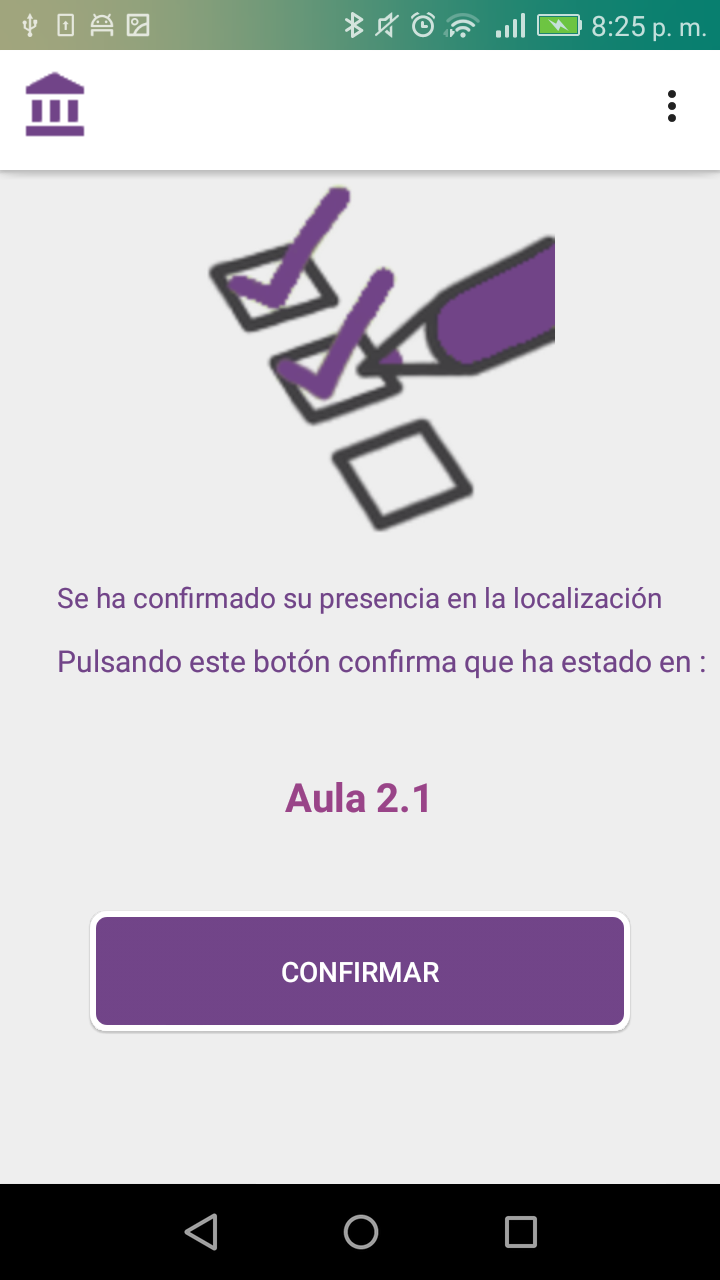
\includegraphics[width=80mm,height=120mm]{ConfirmarAsistencia}
	\caption{Pantalla de confirmación de asistencia en la localización.}
	\label{fig:confirmarAsistencia}
\end{figure}

\lstinputlisting[float, floatplacement=H, caption={Utilizando \textit{ScanFragment} se comprueba que el usuario se encuentra dentro de la zona delimitada.},label={code:scanAtt}]
{listings/scanAtt.java} %% LISTING

\vspace{10mm}

Si no se encuentra en la zona delimitada, igualmente la aplicación muestra su ubicación en el mapa para que pueda corregir su posición. Una vez que acceda al área, se muestra un mensaje de confirmación con el aula en la que se encuentra. En este momento se debe confirmar (Véase Figura \ref{fig:confirmarAsistencia}) pulsando un botón de que el usuario desea registrar la asistencia. Previamente el usuario ha debido introducir sus datos en la aplicación y éstos deben estar almacenados. Estos datos junto con la dirección MAC del dispositivo desde el cual se envía la petición de registro son los que utiliza la aplicación. Otro control es almacenar la hora junto con los demás datos cuando se confirme la asistencia, asegurándonos así de que realmente el usuario ha estado en el aula a dicha hora.


Los datos que se almacenan en el servidor tienen la estructura que se muestra en la Figura \ref{fig:couchDBstucture}, sin embargo esta estructura puede ser fácilmente modificada si se detecta que es necesario añadir más datos.

\begin{figure}[H]
	\centering
	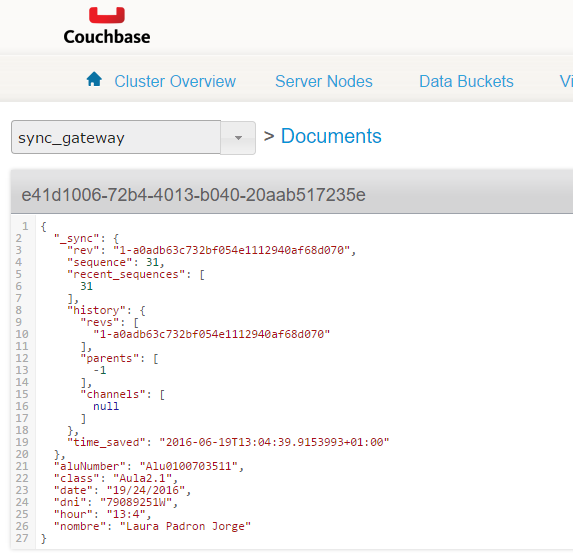
\includegraphics[width=0.6\linewidth]{couchDBstucture}
	\caption{La estructura de los datos del usuario en CouchBase Server.}
	\label{fig:couchDBstucture}
\end{figure}


\subsubsection{Dificultades}

En este caso las dificultades han sido de diversa índole: se ha tenido que configurar un servidor con el que no se había trabajado previamente, se ha tenido que trabajar con la API de preferencias de Android, y había que idear un método que permitiese comprobar de manera fiable que el alumno se encontraba o había estado en la localización a la hora correcta. La configuración del servidor y Sync Gateway ha sido un poco tediosa, pero una vez configurada ha sido muy fácil de utilizar.


\subsubsection{Ampliación}

Para ampliar este caso de uso se deberían incluir nuevos beacons, nuevas imágenes de las localizaciones y nuevas áreas de registro; sin embargo, el envío de datos sería prácticamente el mismo. Si se decidiese cambiar en un futuro los datos a almacenar en el servidor, sería posible sin mucho esfuerzo.

\subsection{Guía a través del campus de la universidad}

\subsubsection{Objetivo}

Este caso de uso se centra en ofrecer una pequeña guía al usuario mostrándole su posición en un edificio y algo de información útil. Para ello hemos tomado a modo de ejemplo el edificio de Matemáticas y Física ya que poseíamos los planos. 

Se han tomado como referencia algunas zonas del edificio y se han creado algunas indicaciones básicas para acompañar la posición en el mapa y los puntos de interés. Es necesario destacar que las pruebas se han realizado utilizando 3 beacons, con lo cual sólo se ha cubierto una pequeña parte del edificio, sin embargo a modo de ejemplo muestra perfectamente las posibilidades de esta tecnología.

\subsubsection{Despliegue}

En este caso, también es necesario utilizar el algoritmo de trilateración. En el listado \ref{code:trilaterate} podemos observar los métodos principales para utilizar la trilateración. Hemos tenido que desplegar 3 beacons en el lugar que queríamos visualizar, en el edificio de Física y Matemáticas en la primera planta, se han colocado en las esquinas de la zona principal, conserjería, cerca de los ascensores y en la entrada a los pasillos principales.


\lstinputlisting[float, floatplacement=H, caption={Los métodos principales para utilizar el algoritmo de trilateración con los beacons, calcular la posición del usuario y dibujar en la imagen.},label={code:trilaterate}]
{listings/trilaterate.java} %% LISTING


\subsubsection{Funcionamiento}


En cuanto se accede al módulo de guía, la aplicación comienza a escanear las inmediaciones buscando beacons. Cuando detecta más de 2 beacons, la aplicación carga la imagen de dicha localización, en este caso el plano del edificio de Física y Matemáticas, una versión reducida para la parte en la que nos encontremos y comprueba que el usuario se encuentra dentro de algunas de las posibles zonas. En cuanto se entre en alguna se mostrará la información relacionada con esta posición. En el estado actual de \BulletPoint{} las acciones de la zona se limitan a mostrar un pequeño texto con información generada teniendo en cuenta que el usuario necesite guiarse en las instalaciones, es decir, no conoce las instalaciones.


Ya que este caso de uso podría ser útil para un rango más amplio de usuarios por su naturaleza de guía, se ha decidido ofrecer soporte en inglés a la hora de mostrar las indicaciones.

\subsubsection{Dificultades}

Las dificultades de este caso de uso radican principalmente en situar al usuario en el edificio. Dentro de un edificio existen muchos factores que pueden distorsionar la calidad de la señal que emite un beacon (paredes, personas, etc.), y por tanto influir en su posición estimada en el mapa. A la hora de enfrentarnos a este problema hemos comprobado que la localización presenta un rango de error y que es necesario darle un margen de tiempo a la aplicación para calcular la posición del usuario. Para intentar paliar esta situación, las áreas en las que se intercambia información con el usuario aparecen resaltadas en el mapa, de esta manera el usuario es capaz de saber con certeza que tiene un área de información e intentar corregir su posición si está interesado. 

\subsubsection{Ampliación}

Para ampliar este caso de uso se deberían incluir nuevos beacons, nuevas imágenes de las localizaciones (exteriores o interiores) y nuevas áreas. Las áreas podrían ofrecer diferentes funcionalidades aparte de la información de la localización.


\subsection{Acceso al parking}

\subsubsection{Objetivo}

El objetivo principal de este caso de uso es permitir a usuario acceder a los aparcamientos universitarios utilizando la aplicación móvil. Actualmente el acceso al parking se formaliza utilizando tarjetas de acceso magnetizadas. El objetivo principal es poder complementar este método con uno más sencillo y más sostenible a largo plazo. 

\subsubsection{Despliegue}

En este caso, también es necesario utilizar el algoritmo de trilateración, por lo que se ha tenido que desplegar 3 beacons en la entrada del parking, se ha utilizado el parking del edificio central, disponiendo los beacons en posiciones previamente seleccionadas como se muestra en la imagen de la Figura \ref{fig:parking}.

\begin{figure}[H]
	\centering
	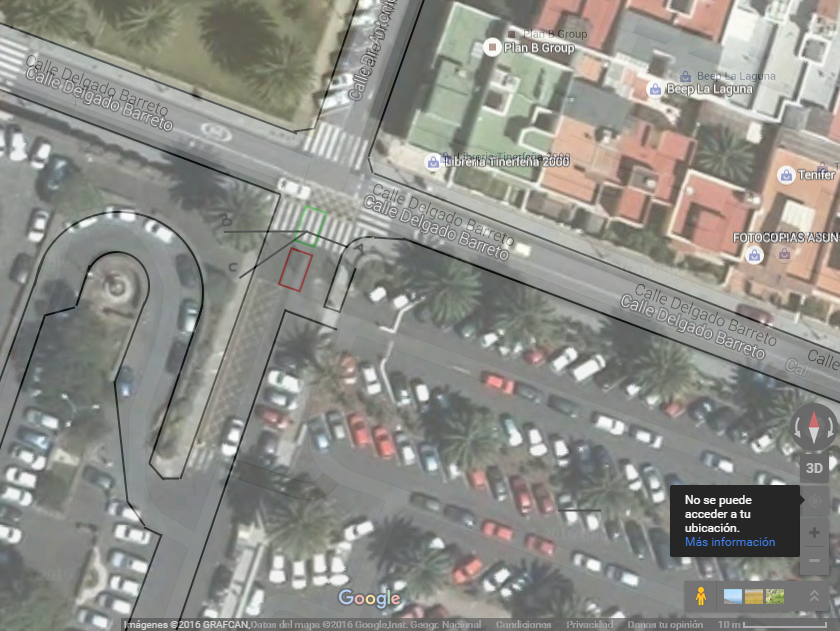
\includegraphics[width=0.7\linewidth]{Parking}
	\label{fig:parking}
	\caption{Se puede apreciar la estructura del parking central. Los puntos A, B y C señalan las posiciones de los beacons.}
\end{figure}

\subsubsection{Funcionamiento}


En cuanto se accede al módulo de parking de \BulletPoint{}, la aplicación muestra una lista con los diferentes aparcamientos y el número de plazas de cada recinto. Esta lista se obtiene mediante una consulta a una API diseñada en colaboración con Alberto Morales, quien se ha encargado de configurar el servicio para facilitar a la aplicación la información necesaria. De la lista de aparcamientos, el usuario ha de seleccionar al que quiere acceder, identificando así la imagen y zonas a dibujar. Esta selección da paso a un escáner que comienza a detectar la posición del usuario y a situarlo en la imagen. Si el usuario se encuentra en una de las zonas designadas para entrar o salir del parking, se lanzará la acción, que en este caso consiste en una petición de apertura contra el servidor. En este caso cada zona posee un identificador de barrera que es el que usa la petición para determinar que barrera debe abrir. 


Por otro lado esta petición debe ir autentificada, para poder acceder, por lo que la aplicación ha negociado previamente un secreto con el servidor que la identifica y le permite realizar la acción de apertura utilizando un número identificativo basado en la MAC del dispositivo de pruebas.


\subsubsection{Dificultades}

En este caso de uso las dificultades han radicado en el hecho de comunicarse con el servidor para realizar las llamadas. La trilateración se ha realizado de la misma manera por lo que no ha habido grandes problemas. Además de estas dificultades, cabe añadir una adicional y es que la seguridad del parking depende del sistema single log in de la ULL, por lo que ha habido que buscar la manera de abordar este tema. Sin embargo, Alberto Morales se ha implicado en todo momento intentado resolver las necesidades de la aplicación de manera óptima, lo que ha sido una gran ayuda.

\subsubsection{Ampliación}

Para ampliar este caso de uso se deberían incluir nuevos beacons, 3 mínimo por cada recinto, nuevas imágenes de las localizaciones (exteriores o interiores) y nuevas áreas; Las áreas serían esenciales para definir las acciones de apertura de las barreas. Si las zonas acaban siendo muchas, sería recomendable crear una base de datos  para almacenar las localizaciones, las zonas y las imágenes a cargar.

\section{Despliegue}

El despliegue de estos dispositivos es variable como hemos podido comprobar con los distintos casos de uso. Sin embargo hay ciertas consideraciones comunes a en todos los casos, si lo que deseamos es un sistema que detecte entradas y salidas, independientemente de la posición exacta del usuario, simplemente necesitaremos un único beacon como regla general. 


Sin embargo, si se pretende conocer la localización más precisa del usuario necesitaremos recurrir a un método como la trilateración \cite{URL::trilateracion}. Serán necesarios un mínimo de 3 beacons. Incrementando el número de beacons es posible aumentar la precisión con la que se percibe la posición del usuario. El algoritmo no es totalmente exacto, puesto que depende de las distancias calculadas a los beacons, sin embargo estas distancias pueden variar. Existen diversos factores que pueden influir en la calidad de la señal del Bluetooth y por tanto distorsionar estas distancias, entre otros factores podemos destacar principalmente:


\begin{itemize}
\item Físicos:  paredes, personas o elementos del entorno principalmente.
\item Intangibles: interferencias con otras ondas.
\item Configurables: la intensidad de la señal y por tanto su rango es configurable.
\end{itemize}


Todos estos factores han de ser tomados en cuenta a la hora de realizar el despliegue de los beacons. Otro factor a tener en cuenta es la altura. Los dispositivos es recomendables levantarlos cierta altura sobre el nivel del suelo. A la hora de probarlos se ha intentado, en la medida de lo posible, mantenerlos a un nivel elevado sobre la altura de las personas y siempre intentando mantener esta medida de altura para los diferentes beacons. En cuanto al despliegue de la aplicación, el código fuente de \BulletPoint{} se encuentra disponible para su descarga en \cite{URL::repositorioAplicacion}, bajo licencia Creative Commons Reconocimiento-NoComercial-CompartirIgual 4.0 Internacional \cite{URL::licencia}.





